\documentclass[10pt,reqno]{amsart}

\usepackage[T1]{fontenc}
\usepackage{lmodern}
\usepackage{amsmath}
\usepackage{amssymb}
\usepackage{mathtools}
\usepackage{booktabs}
\usepackage{array}
\usepackage{enumitem}
\usepackage{microtype}
\usepackage{xr-hyper}
\usepackage{hyperref}
\usepackage{url}
\usepackage{xcolor}
\usepackage{placeins}
\usepackage{tikz}
\usepackage{tikz-cd}
\usepackage{etoolbox}
\AtBeginEnvironment{thebibliography}{\small\setlength{\itemsep}{0pt}}
\usepackage{longtable}
\usetikzlibrary{arrows.meta,calc}
\definecolor{pathblue}{RGB}{30,84,139}
\definecolor{pathorange}{RGB}{177,83,23}
\definecolor{pathteal}{RGB}{28,117,108}

\hypersetup{
  hidelinks,
  pdftitle={Technical Supplement to Topological Semantics for Scoped Computational Paths},
  pdfauthor={Arthur Freitas Ramos, Ruy J. G. B. de Queiroz, Anjolina Grisi de Oliveira, and Tiago M. L. de Veras},
  pdfsubject={Topological semantics for scoped computational-path rewrite presentations},
  pdfkeywords={computational paths, rewriting, fundamental groupoid, quotient topology, topological groupoid}
}

\emergencystretch=3em
\allowdisplaybreaks

\theoremstyle{definition}
\newtheorem{definition}{Definition}[section]
\newtheorem{example}[definition]{Example}
\newtheorem{construction}[definition]{Construction}
\theoremstyle{plain}
\newtheorem{theorem}[definition]{Theorem}
\newtheorem{lemma}[definition]{Lemma}
\newtheorem{proposition}[definition]{Proposition}
\newtheorem{corollary}[definition]{Corollary}
\theoremstyle{remark}
\newtheorem{remark}[definition]{Remark}

\newcommand{\Path}{\mathsf{Path}}
\newcommand{\Trace}{\mathsf{Trace}}
\newcommand{\Step}{\mathsf{Step}}
\newcommand{\RwEq}{\mathrel{\simeq_{\!\mathcal P}}}
\newcommand{\PiOne}{\Pi_1}
\newcommand{\Fin}{\mathrm{fin}}
\newcommand{\Ord}{\mathrm{ord}}
\newcommand{\Top}{\mathsf{Top}}
\newcommand{\Z}{\mathbb Z}
\newcommand{\N}{\mathbb N}
\newcommand{\Circle}{\mathbb R/\mathbb Z}
\urlstyle{tt}
\newcommand{\LeanName}[1]{\path{#1}}

\title[Topological Semantics for Scoped Computational Paths]
  {Technical Supplement to Topological Semantics for Scoped Computational Paths}

\author{Arthur Freitas Ramos}

\author{Ruy J. G. B. de Queiroz}

\author{Anjolina Grisi de Oliveira}

\author{Tiago M. L. de Veras}

\renewcommand{\shortauthors}{Ramos et al.}

\subjclass[2020]{Primary 22A22, 54B15; Secondary 03B38, 55Q05, 68V20, 54B30}
\keywords{computational paths, rewriting, fundamental groupoid, quotient topology, topological groupoid}

\externaldocument[main-]{../../output/paper35/main}[main-35-pages.pdf]
\begin{document}

\raggedbottom

\renewcommand{\thesection}{S\arabic{section}}
\begin{abstract}
This supplement retains the full construction proofs, classical examples,
formalization maps, and artifact history accompanying the
\href{main-35-pages.pdf}{main paper}. Its theorem numbering is local to the
supplement. References to omitted main-paper sections and results link to
that paper. The earlier \href{geometric-rose-all-loops.pdf}{full manuscript}
is preserved separately.
\end{abstract}
\maketitle

\section{Construction calculations and geometric illustrations}
Use the signed-word, endpoint and topology conventions of the main paper.
The following are the complete proofs of its shortened construction lemmas.
The diagrams retain the accompanying geometric explanations.

\begin{lemma}[continuity of trace realization]
\label{lem:trace-realization-continuous}
The equal-slot realization map
\[
  |\cdot|:\mathsf{Tr}_{\mathcal P}\longrightarrow X^I
\]
is continuous for the coproduct trace topology.
\end{lemma}

\begin{proof}
On the zero-letter component $W_0=X$, the realization is the constant-path
map.  Its adjoint $X\times I\to X$, $(a,t)\mapsto a$, is continuous, so the
compact-open exponential law gives continuity into $X^I$.  Fix $n\geq1$.
For each $1\leq i\leq n$, the closed slot
\[
  C_i=W_n\times[(i-1)/n,i/n]\subseteq W_n\times I
\]
supports the continuous formula
\[
  (p,t)\longmapsto
  \widetilde\rho(e_i(p))(nt-i+1),
\]
where $e_i:W_n\to\widetilde E$ is the $i$th coordinate.  Continuity follows
from the continuity of $\widetilde\rho$ and of evaluation for the compact-open
topology.  On a
common boundary $t=i/n$, the two formulas agree because composability gives
\(\widetilde t(e_i)=\widetilde s(e_{i+1})\).  The pasting lemma therefore gives a continuous adjoint
\(W_n\times I\to X\).  Since $I$ is compact Hausdorff, the compact-open
exponential law gives a continuous map $W_n\to X^I$.  The coproduct
universal property now assembles these component maps into the displayed
realization map.
\end{proof}

\begin{lemma}[continuity of coherent operations]\label{lem:coherent-operations-continuous}
For either $*=\mathrm{tr}$ or $*=\mathrm{obs}$, let $\iota:X\to T_*$ send
$a$ to the coherent identity $(1_a,c_a)$, let $\sigma:T_*\to T_*$ send
$(p,\gamma)$ to
$(p^{-1},\gamma^{-1})$, and let
\[
  \mu_*:T_*^{(2)}\longrightarrow T_*,
  \qquad ((p,\gamma),(q,\delta))\longmapsto
    (p;q,\gamma\star_{\ell(p),\ell(q)}\delta),
\]
where the weighted operation uses the discrete trace lengths.  Then all three
maps are continuous.
\end{lemma}

\begin{proof}
For $T_{\mathrm{obs}}$, it is enough to check continuity after applying
$\kappa_{\mathrm{obs}}$.  The three resulting observable codes are respectively
\[
  (a,a,0,c_a,c_a),
\quad
  (t(p),s(p),\ell(p),|p|^{-1},\gamma^{-1}),
\]
and, on the composable pullback,
\[
  \bigl(s(p),t(q),\ell(p)+\ell(q),
    |p|\star_{\ell(p),\ell(q)}|q|,
    \gamma\star_{\ell(p),\ell(q)}\delta\bigr).
\]
The first is continuous because constant paths depend continuously on $a$;
the second uses reversal on $X^I$; and the third uses addition on the discrete
length coordinate and continuity of the weighted operation on each fixed
length component.  Each code depends continuously only on the observable
codes of the input(s), so the initial-topology criterion proves continuity of
all three operations.  For $T_{\mathrm{tr}}$, the corresponding first
coordinates are the continuous word maps
$a\mapsto 1_a$, $p\mapsto p^{-1}$, and $(p,q)\mapsto p;q$ on the trace
carrier; the second coordinates are the same continuous path operations just
used.  The initial-topology criterion for $\kappa_{\mathrm{tr}}$ therefore
proves continuity in the trace-sensitive topology as well.  Reversal and
weighted concatenation preserve the coherence predicate by reversing and
concatenating the endpoint-fixed homotopies.  The Lean development flattens
the parenthesized internal trace to a signed word so that these
first-coordinate maps can be checked.
\end{proof}

\begin{lemma}[weighted concatenation invariance]
\label{lem:weighted-concat-invariance}
Let $\alpha\simeq_{\partial I}\alpha'$ and
$\beta\simeq_{\partial I}\beta'$ be endpoint-fixed homotopies of composable
paths.  Write $c_x$ for the constant path at $x$, and assume explicitly that
\[
\begin{aligned}
m=0&\Rightarrow \alpha(0)=\alpha(1)\ \text{and}\ \alpha\simeq_{\partial I}c_{\alpha(0)},\\
n=0&\Rightarrow \beta(0)=\beta(1)\ \text{and}\ \beta\simeq_{\partial I}c_{\beta(0)},\\
m'=0&\Rightarrow \alpha'(0)=\alpha'(1)\ \text{and}\ \alpha'\simeq_{\partial I}c_{\alpha'(0)},\\
n'=0&\Rightarrow \beta'(0)=\beta'(1)\ \text{and}\ \beta'\simeq_{\partial I}c_{\beta'(0)}.
\end{aligned}
\]
For arbitrary
$m,n,m',n'\in\N$, with the zero-length conventions above,
\[
  \alpha\star_{m,n}\beta
  \simeq_{\partial I}
  \alpha'\star_{m',n'}\beta'.
\]
\end{lemma}

\begin{proof}
When all four weights are positive, let $\lambda_{m,n}:[0,1]\to[0,1]$ be
the piecewise-linear endpoint-fixing homeomorphism that maps
$m/(m+n)$ to $1/2$ and is linear on the two sides.  Explicitly,
\[
 \lambda_{m,n}(t)=
 \begin{cases}
   \dfrac{m+n}{2m}t,
     &0\leq t\leq\dfrac{m}{m+n},\\[6pt]
   \dfrac12+\dfrac{m+n}{2n}\left(t-\dfrac{m}{m+n}\right),
     &\dfrac{m}{m+n}\leq t\leq1.
 \end{cases}
\]
Then
\[
  \alpha\star_{m,n}\beta
  =(\alpha\star_{1,1}\beta)\circ\lambda_{m,n}.
\]
The straight-line homotopy $(1-u)\lambda_{m,n}+u\lambda_{m',n'}$ fixes $0$ and
$1$, so changing the breakpoint gives an endpoint-fixed reparametrization
homotopy.  Horizontal concatenation of the
given homotopies at the common breakpoint $1/2$ gives
\[
  \alpha\star_{1,1}\beta
  \simeq_{\partial I}
  \alpha'\star_{1,1}\beta'.
\]
Combining these homotopies proves the claim when all weights are positive.
If a weight is zero, first use the corresponding zero-slot hypothesis to replace
the corresponding factor by the constant path at its endpoint.  Such a factor
has coinciding endpoints by the displayed hypothesis, so the stated
convention then deletes that constant factor.  When the zero/nonzero status
changes between the two sides, this replacement inserts or removes the factor
up to endpoint-fixed homotopy.  The remaining positive-weight factors are
handled by the preceding reparametrization argument; when both weights are
zero, the convention yields the common endpoint constant.  Thus all
zero-length cases follow as well.
\end{proof}

\begin{lemma}[backtracking contracts in every space]
\label{lem:backtracking}
For any continuous path $\alpha:I\to X$, the formula
\[
 H(u,t)=\alpha\!\left(\min\{2t,\,2(1-t),\,1-u\}\right)
 \qquad (u,t\in I)
\]
is an endpoint-fixed homotopy from
$\alpha\star_{1,1}\alpha^{-1}$ to $c_{\alpha(0)}$.
\end{lemma}
\begin{proof}
The minimum is a continuous map $I^2\to I$, so $H$ is continuous.
At $u=0$ its argument is the triangular function
$\min\{2t,2(1-t)\}$, which traverses $\alpha$ and then retraces it.
At $u=1$ it is identically zero, and for every $u$ its values at
$t=0,1$ are zero.  These are the required boundary conditions.
Applying the same construction to $\alpha^{-1}$ proves the other inverse law.
\end{proof}

\subsection*{Supplementary construction diagrams}
\begin{figure}[htbp]
\centering
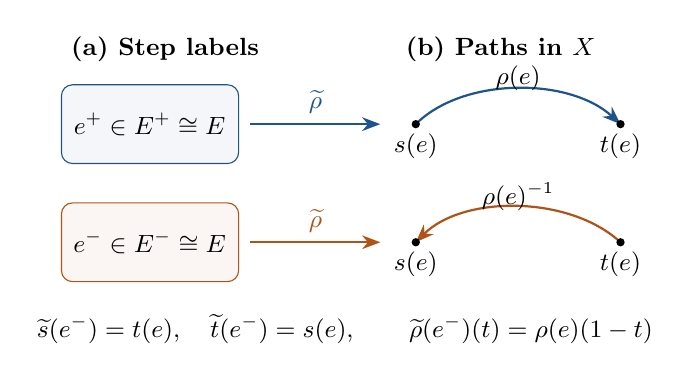
\begin{tikzpicture}[font=\small,>=Stealth]
\node[anchor=west,font=\small\bfseries] at (0,2.4) {(a) Step labels};
\draw[rounded corners,fill=pathblue!5,draw=pathblue] (0,0.95) rectangle (2.25,1.95);
\draw[rounded corners,fill=pathorange!5,draw=pathorange] (0,-0.55) rectangle (2.25,0.45);
\node at (1.12,1.45) {$e^+\in E^+\cong E$};
\node at (1.12,-0.05) {$e^-\in E^-\cong E$};
\draw[->,pathblue,thick] (2.4,1.45) -- node[above] {$\widetilde\rho$} (4.05,1.45);
\draw[->,pathorange,thick] (2.4,-0.05) -- node[above] {$\widetilde\rho$} (4.05,-0.05);
\node[anchor=west,font=\small\bfseries] at (4.25,2.4) {(b) Paths in $X$};
\draw[->,pathblue,thick] (4.5,1.45) .. controls (5.1,2.05) and (6.45,2.05) .. (7.1,1.45);
\fill (4.5,1.45) circle (1.5pt) node[below] {$s(e)$};
\fill (7.1,1.45) circle (1.5pt) node[below] {$t(e)$};
\node at (5.8,2.03) {$\rho(e)$};
\draw[<-,pathorange,thick] (4.5,-0.05) .. controls (5.1,0.55) and (6.45,0.55) .. (7.1,-0.05);
\fill (4.5,-0.05) circle (1.5pt) node[below] {$s(e)$};
\fill (7.1,-0.05) circle (1.5pt) node[below] {$t(e)$};
\node at (5.8,0.53) {$\rho(e)^{-1}$};
\node[align=center] at (3.6,-1.15) {$\widetilde s(e^-)=t(e),\quad
 \widetilde t(e^-)=s(e),\qquad
 \widetilde\rho(e^-)(t)=\rho(e)(1-t)$};
\end{tikzpicture}
\caption{Formal reversal changes the direction of a represented path and
leaves the topology of the step space unchanged.  The two curves depict the same geometric
route traversed in opposite directions.  Endpoint maps take values in $X$;
the realization map takes values in $X^I$.}
\label{fig:oriented-steps}
\end{figure}


\begin{figure}[htbp]
\centering
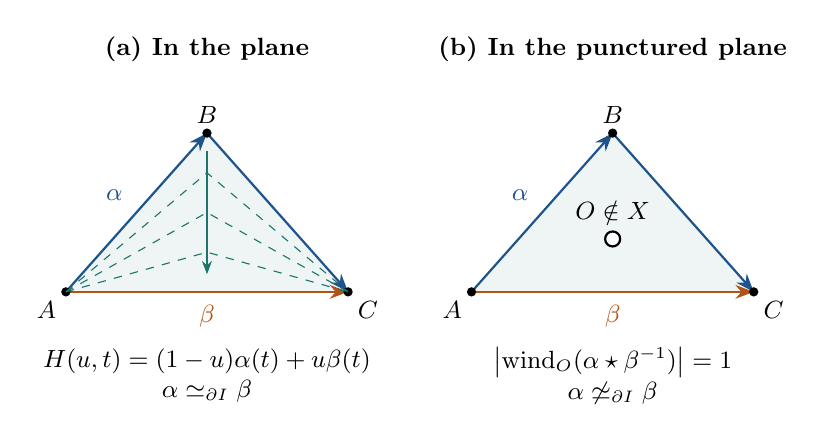
\begin{tikzpicture}[font=\small,>=Stealth,scale=1.12]
\foreach \x/\lab in {0/{(a) In the plane},4.6/{(b) In the punctured plane}} {
 \begin{scope}[xshift=\x cm]
 \node[font=\small\bfseries] at (1.6,2.75) {\lab};
 \fill[pathteal!7] (0,0) -- (1.6,1.8) -- (3.2,0) -- cycle;
 \draw[->,pathblue,thick] (0,0) -- (1.6,1.8);
 \draw[->,pathblue,thick] (1.6,1.8) -- (3.2,0);
 \draw[->,pathorange,thick] (0,0) -- (3.2,0);
 \fill (0,0) circle(1.5pt) node[below left] {$A$};
 \fill (1.6,1.8) circle(1.5pt) node[above] {$B$};
 \fill (3.2,0) circle(1.5pt) node[below right] {$C$};
 \node[pathblue] at (0.55,1.1) {$\alpha$};
 \node[pathorange] at (1.6,-0.28) {$\beta$};
 \end{scope}
}
\foreach \h in {0.45,0.9,1.35} {
 \draw[pathteal,dashed] (0,0) -- (1.6,\h) -- (3.2,0);
}
\draw[->,pathteal] (1.6,1.6) -- (1.6,0.2);
\draw[fill=white,thick] (6.2,0.6) circle(0.085);
\node[anchor=south,inner sep=1pt] at (6.2,0.77) {$O\notin X$};
\node[align=center] at (1.6,-0.95) {$H(u,t)=(1-u)\alpha(t)+u\beta(t)$\\
 $\alpha\simeq_{\partial I}\beta$};
\node[align=center] at (6.2,-0.95) {$\left|\operatorname{wind}_{O}
 (\alpha\star\beta^{-1})\right|=1$\\
 $\alpha\not\simeq_{\partial I}\beta$};
\end{tikzpicture}
\caption{Coherence requires a homotopy inside the chosen ambient space.
Left: intermediate broken paths move $B$ to the segment $AC$, keeping $A,C$
fixed.  Right: deleting the interior point $O=(0,\tfrac13)$ prevents any
such homotopy, although both boundary paths remain continuous.
For $|p|=\alpha$, $(p,\beta)$ is coherent only in the left-hand example.
The shaded triangle is available in (a), but is not a filling in (b).}
\label{fig:coherence}
\end{figure}


\begin{figure}[htbp]
\centering
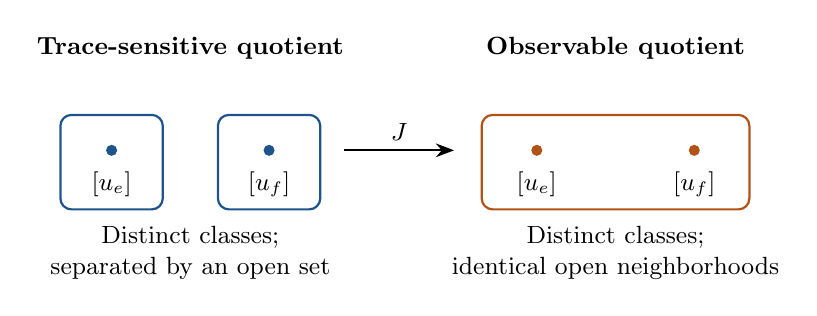
\begin{tikzpicture}[font=\small,>=Stealth]
\node[font=\small\bfseries] at (0,1.6) {Trace-sensitive quotient};
\node[font=\small\bfseries] at (5.4,1.6) {Observable quotient};
\draw[pathblue,thick,rounded corners] (-1.65,-0.45) rectangle (-0.35,0.75);
\draw[pathblue,thick,rounded corners] (0.35,-0.45) rectangle (1.65,0.75);
\fill[pathblue] (-1,0.3) circle (2pt);
\fill[pathblue] (1,0.3) circle (2pt);
\node[below] at (-1,0.15) {$[u_e]$};
\node[below] at (1,0.15) {$[u_f]$};
\draw[pathorange,thick,rounded corners] (3.7,-0.45) rectangle (7.1,0.75);
\fill[pathorange] (4.4,0.3) circle (2pt);
\fill[pathorange] (6.4,0.3) circle (2pt);
\node[below] at (4.4,0.15) {$[u_e]$};
\node[below] at (6.4,0.15) {$[u_f]$};
\draw[->,thick] (1.95,0.3) -- (3.35,0.3) node[midway,above] {$J$};
\node[align=center] at (0,-1) {Distinct classes;\\separated by an open set};
\node[align=center] at (5.4,-1) {Distinct classes;\\identical open neighborhoods};
\end{tikzpicture}
\caption{The two quotients identify the same arrows and differ only in
their topology.
In Example~\ref{main-ex:quotient-topology-separation}, both steps realize the
same nonconstant circle loop, but their signed-count values differ. The map $J$
preserves both scoped classes.  In the observable quotient every open set
containing either class contains both.  Boxes illustrate separation properties
only; the shared box is not asserted to be an open two-point subset.}
\label{fig:same-geometry}
\end{figure}


\begin{figure}[htbp]
\centering
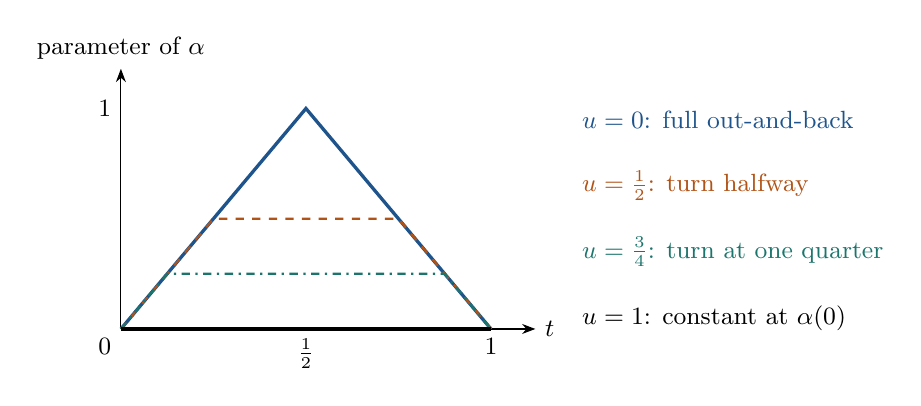
\begin{tikzpicture}[font=\small,>=Stealth,x=4.7cm,y=2.8cm]
\draw[->] (0,0) -- (1.12,0) node[right] {$t$};
\draw[->] (0,0) -- (0,1.18) node[above] {parameter of $\alpha$};
\draw[pathblue,very thick] (0,0) -- (0.5,1) -- (1,0);
\draw[pathorange,thick,dashed] (0,0) -- (0.25,0.5) -- (0.75,0.5) -- (1,0);
\draw[pathteal,thick,dash dot] (0,0) -- (0.125,0.25) -- (0.875,0.25) -- (1,0);
\draw[black,very thick] (0,0) -- (1,0);
\node[below left] at (0,0) {$0$};
\node[below] at (0.5,0) {$\tfrac12$};
\node[below] at (1,0) {$1$};
\node[left] at (0,1) {$1$};
\node[pathblue,anchor=west] at (1.22,0.95) {$u=0$: full out-and-back};
\node[pathorange,anchor=west] at (1.22,0.65) {$u=\tfrac12$: turn halfway};
\node[pathteal,anchor=west] at (1.22,0.35) {$u=\tfrac34$: turn at one quarter};
\node[anchor=west] at (1.22,0.05) {$u=1$: constant at $\alpha(0)$};
\end{tikzpicture}
\caption{Backtracking cancellation as an explicit homotopy.
The plotted function is $r_u(t)=\min\{2t,2(1-t),1-u\}$;
the actual path is $H(u,t)=\alpha(r_u(t))$.
As $u$ increases, the turning point retreats along $\alpha$ and the path
waits there before returning.  All intermediate paths stay in $\alpha(I)$,
so even a hole surrounded by $\alpha$ cannot obstruct this cancellation.}
\label{fig:backtracking}
\end{figure}


\begin{figure}[htbp]
\centering
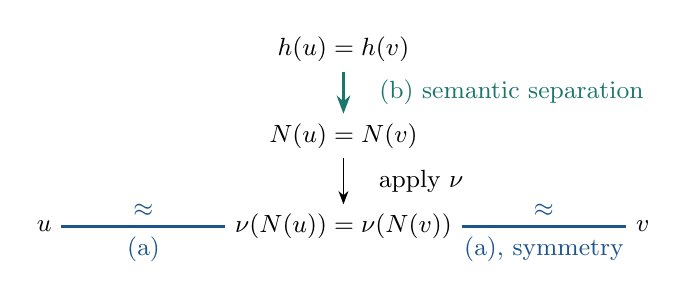
\begin{tikzpicture}[font=\small,>=Stealth]
\node (geo) at (0,2) {$h(u)=h(v)$};
\node (code) at (0,0.9) {$N(u)=N(v)$};
\draw[->,pathteal,thick] (geo) -- (code)
 node[midway,right] {\quad(b) semantic separation};
\node (common) at (0,-0.25) {$\nu(N(u))=\nu(N(v))$};
\draw[->] (code) -- (common) node[midway,right] {\quad apply $\nu$};
\node (u) at (-3.8,-0.25) {$u$};
\node (v) at (3.8,-0.25) {$v$};
\draw[pathblue,thick] (u) -- (common)
 node[midway,above] {$\approx$} node[midway,below] {(a)};
\draw[pathblue,thick] (common) -- (v)
 node[midway,above] {$\approx$} node[midway,below] {(a), symmetry};
\end{tikzpicture}
\caption{A normal-form certificate proves completeness by two different
means: syntactic normalization (a) connects each trace to its chosen normal
representative; semantic separation (b) forces the two codes to agree.
The bottom row is then scoped transitivity, yielding $u\approx v$.
The arrows are logical steps and assume nothing about continuity of $N$ or
$\nu$.}
\label{fig:normal-form}
\end{figure}


\section{Universal projection lemmas}
The universal presentation and its scoped relation are those of the main
paper. These projection and fixed-endpoint arguments supplement the full
ordinary-composition proof retained there.

\begin{lemma}[coherent-path quotient identification]
\label{lem:coherent-path-quotient-identification}
For the universal presentation, the projection
\[
  \pi:T_{\mathcal U_X}\longrightarrow X^I,
  \qquad \pi(p,\gamma)=\gamma,
\]
is a continuous quotient map.  Consequently, the quotient of
$T_{\mathcal U_X}$ by endpoint-fixed homotopy of the chosen representative is
canonically homeomorphic to the usual quotient-topologized path-class space
\[
  \Pi_1^q(X)=X^I/{\simeq_{\partial I}},
\]
with the endpoint maps retained.
\end{lemma}

\begin{proof}
For $T_{\mathrm{obs}}$, continuity of $\pi$ is immediate from the fifth
coordinate of $\kappa_{\mathrm{obs}}$.  For $T_{\mathrm{tr}}$, it is the
restriction of the second projection
$\mathsf{Tr}_{\mathcal P}\times X^I\to X^I$.  Every $\gamma\in X^I$ has the
coherent representative
\[
  \sigma(\gamma)=(\langle\gamma\rangle,\gamma),
\]
where $\langle\gamma\rangle$ is the one-letter universal trace and the
coherence is the constant endpoint-fixed homotopy.  The map $\sigma$ is
continuous on the one-letter coproduct component for $T_{\mathrm{tr}}$; it is
also continuous for $T_{\mathrm{obs}}$ because its observable code is built
continuously from $\gamma$.  Since $\pi\sigma=\mathrm{id}$, if
$\pi^{-1}(U)$ is open then
$U=\sigma^{-1}(\pi^{-1}(U))$ is open.  Thus $\pi$ is quotient.  The general quotient-factorization
lemma applied to the homotopy relation now induces mutually inverse
continuous maps between the two displayed quotient spaces.
\end{proof}

\begin{lemma}[fiberwise coherent-path quotient]
\label{lem:fiberwise-coherent-path-quotient}
Fix $a,b\in X$, and let
\[
  X^I(a,b)=\{\gamma\in X^I:\gamma(0)=a,\ \gamma(1)=b\}
\]
carry its subspace topology.  For $*=\mathrm{tr},\mathrm{obs}$, define the
coherent carrier with these fixed endpoints
\[
  T_{\mathcal U_X}^{*}(a,b)=
  \{(p,\gamma)\in T_{\mathcal U_X}^{*}:s(p)=a,\ t(p)=b\}
\]
with its own subspace topology, and define
$G_{\mathcal U_X}^{*}(a,b)$ to be its quotient by scoped equivalence, with
the quotient topology.  The restricted projection
\[
  \pi_{a,b}^{*}:T_{\mathcal U_X}^{*}(a,b)\longrightarrow X^I(a,b)
\]
is quotient.  Hence $G_{\mathcal U_X}^{*}(a,b)$ is canonically homeomorphic
to the endpoint-fixed homotopy quotient of $X^I(a,b)$.
\end{lemma}

\begin{proof}
The projection is continuous for either representative topology.  Its
one-letter section
\[
  \sigma_{a,b}(\gamma)=(\langle\gamma\rangle,\gamma)
\]
lands in the fixed endpoint fiber and is continuous by the same coordinate
argument as in Lemma~\ref{lem:coherent-path-quotient-identification}.
If $(\pi_{a,b}^{*})^{-1}(U)$ is open, then
$U=\sigma_{a,b}^{-1}((\pi_{a,b}^{*})^{-1}(U))$ is open.  Thus the restricted
projection is quotient without appealing to a restriction theorem for the
global projection.  In the universal presentation, scoped equivalence on this
fiber is exactly endpoint-fixed homotopy, so quotient factorization gives the
claimed homeomorphism.
\end{proof}

\begin{figure}[htbp]
\centering
\begin{tikzcd}[column sep=5em,row sep=4em,
 every label/.append style={font=\normalsize},
 every cell/.append style={font=\large}]
 X^I \arrow[r,shift left=1ex,"\sigma"] \arrow[d,"q_I"']
 & T_{\mathcal U_X}^{*} \arrow[l,shift left=1ex,"\pi"] \arrow[d,"q_*"] \\
 \Pi_1^q(X) \arrow[r,shift left=1ex,"\overline\sigma"]
 & G_{\mathcal U_X}^{*} \arrow[l,shift left=1ex,"\overline\pi"]
\end{tikzcd}

\smallskip
\(\displaystyle
 \pi\sigma=\mathrm{id}_{X^I},\qquad
 G_{\mathcal U_X}^{\mathrm{tr}}\cong\Pi_1^q(X)
 \cong G_{\mathcal U_X}^{\mathrm{obs}}.
\)
\caption{The universal one-letter section supplies the topology, and the
universal rules supply the equivalence relation.  Here
$*\in\{\mathrm{tr},\mathrm{obs}\}$ and
$\sigma(\gamma)=(\langle\gamma\rangle,\gamma)$; $q_I$ is the homotopy
quotient map.  The lower maps are induced by $\sigma$ and $\pi$.
The upper maps are continuous, with $\pi\sigma=\mathrm{id}$, so $\pi$ is
quotient.  Agreement of scoped and homotopy relations makes the lower maps
mutually inverse homeomorphisms.  Under these identifications, $J_{\mathcal U_X}$
is the identity on path classes.}
\label{fig:universal-section}
\end{figure}


\section{Circle, torus and product proofs}
These arguments use the finite presentations and endpoint conventions of
Section~\ref{main-sec:circle-torus} of the main paper. The global based-arrow
subspace comparison is established separately from the based-carrier quotient.

\begin{theorem}[circle winding classification]
\label{thm:circle-winding}
The finite-generator scoped presentation is geometrically complete on the
based loop fiber, and winding number is a group isomorphism and a
homeomorphism
\[
  L\cong\Z,
\]
where $\Z$ is discrete.
Moreover, the inverse realization comparison
\[
  S_0:L\xrightarrow{\ \cong\ }G_{\mathcal P}(0,0)
\]
is a homeomorphism.  In particular the scoped presentation is
nondegenerate: the images of the zero and one winding loops are distinct.
\end{theorem}

\begin{proof}
A based loop has a unique lift to $\mathbb R$ starting at $0$.
Its endpoint is an integer, and endpoint-fixed homotopy preserves that
integer.  Straight-line interpolation of the lift with $t\mapsto tn$
shows that every loop of winding $n$ is homotopic to $\lambda_n$.
The lift of a concatenation is the first lift followed by a translate of the
second, so winding is additive.  Thus winding identifies $L$ with $\mathbb Z$
as groups.

The finite-generator reduction lemma in the main paper sends every trace to $c_n$, where $n$ is
its winding number, so the normal-form criterion gives geometric
completeness.  Explicitly, $S_0$ sends a loop class of winding $n$ to
$q(c_n,\lambda_n)$.  Every scoped class has this form by normalization,
and soundness prevents different windings from giving the same scoped
class.  Hence $S_0$ is inverse to realization.  In particular, the zero
and one winding classes are distinct.



It remains to prove continuity of $S_0$.  Give $\mathbb T$ its standard
quotient metric.  If two based loops $\gamma,\delta$ are uniformly less
than $1/2$ apart, their difference has a unique continuous representative
$d:I\to(-1/2,1/2)$, with $d(0)=d(1)=0$.
Then $\gamma(t)+[u\,d(t)]$ joins them relative to endpoints.
Compact-open and uniform topologies agree here since $I$ is compact and
$\mathbb T$ is metric.  Winding is therefore locally constant and descends
continuously from $L$ to discrete $\Z$.
Choosing $(c_n,\lambda_n)$ for each $n$ gives a continuous map from
discrete $\Z$ to the coherent carrier and then to its scoped quotient.
This constructs $S_0$ continuously; projection to the chosen loop
supplies its continuous inverse on the fixed-endpoint quotient.

\enlargethispage{2\baselineskip}
To check the topology inherited by $G_{\mathcal P}(0,0)$ from the
\emph{global} scoped arrow space, consider a coherent raw representative
with source $x$ and chosen geometric loop $\gamma$. Every trace in this
finite presentation has equal source and target. Define
\[
  W(x,\gamma)=\operatorname{wind}
    \bigl(t\mapsto\gamma(t)-x\bigr).
\]
Translation of a variable-basepoint loop to zero is continuous in the
compact-open topology. The observable raw topology includes both $x$ and
$\gamma$, and winding is locally constant on based loops, so $W$ is
continuous on the full raw carrier. Scoped equivalence preserves the
source and gives an endpoint-fixed homotopy of the chosen loops. Thus $W$
descends continuously to the global arrow quotient. On the based subspace
it is ordinary winding. Normal-form completeness makes this restriction
injective, while the classes of $(c_n,\lambda_n)$ make it surjective. Its
inverse is continuous because $\mathbb Z$ is discrete. This proves the
claimed homeomorphism for the actual subspace topology without restricting
a quotient map. The based loop-class quotient is discrete; the loop space
itself need not be.
\end{proof}

\begin{theorem}[torus winding classification]
\label{thm:torus-winding}
For the torus $\mathbb T^2$, the coordinate winding pair is a group
isomorphism and a homeomorphism
\[
  L_{\mathbb T^2}\cong\Z\times\Z,
\]
where $\Z\times\Z$ is discrete.
The finite-generator scoped presentation is geometrically complete on the
based loop fiber.  Moreover, the inverse realization comparison
\[
  S_{\mathbb T^2}:L_{\mathbb T^2}\xrightarrow{\ \cong\ }
  G_{\mathcal P}((0,0),(0,0))
\]
is a homeomorphism.
\end{theorem}

\begin{proof}
The universal cover is the product map
\[
  \mathbb R^2\longrightarrow\mathbb T^2,
  \qquad (x,y)\longmapsto([x],[y]).
\]
The lift of a based loop has endpoint $(m,n)\in\mathbb Z^2$, and endpoint-fixed
homotopy preserves this pair.  Conversely, the two coordinate projections of
any based torus loop are circle loops; the circle lifting theorem gives
endpoint-fixed homotopies to the standard loops of windings $m$ and $n$.
Taking their product gives a homotopy to the simultaneous loop $d_{m,n}$;
Lemma~\ref{main-lem:torus-sequential} then gives a homotopy to the sequential
realization $|a^m;b^n|$.  Thus the coordinate winding pair classifies
geometric loops, and it is additive because each coordinate winding is.  The signed-word reduction in the main paper gives the corresponding scoped
derivation, so the normal-form criterion proves geometric completeness.
Projection from coherent representatives to their chosen loops induces
the continuous realization comparison.  The local-constancy argument
constructs its inverse continuously: each coordinate
winding number is locally constant by the circle argument.  The winding pair thus
descends continuously to discrete $\Z^2$, and the map
$(m,n)\mapsto(a^m;b^n,d_{m,n})$ is continuous because its domain is discrete.
Lemma~\ref{main-lem:torus-sequential} ensures that each pair is coherent.
Composing these maps with the scoped quotient map gives $S_{\mathbb T^2}$.
For the topology inherited from the global scoped arrow space, translate
each variable-basepoint torus loop $\gamma$ by its source $x$ and take the
two coordinate windings of $t\mapsto\gamma(t)-x$. This gives a continuous
$\mathbb Z^2$-valued map on the global quotient: translation and winding
are continuous, and scoped soundness makes the value independent of the
representative. Its restriction to the based subspace is bijective by the
normal form above, with continuous inverse from discrete $\mathbb Z^2$.
This proves the stated subspace homeomorphism. As for the circle, the
loop space itself is not asserted to be discrete.
\end{proof}

\begin{theorem}[product closure of based completeness]
\label{thm:product-completeness}
Suppose $\mathcal P$ is geometrically complete on the based-loop fiber at
$x\in X$ and $\mathcal Q$ is geometrically complete on the based-loop
fiber at $y\in Y$.  Then $\mathcal P\boxtimes\mathcal Q$ is geometrically
complete on the based-loop fiber at $(x,y)$.
\end{theorem}

\begin{proof}
Induct on a product trace.  Identity traces and single letters are already
sorted after inserting a unit trace.  For a concatenation, first sort both
parts, then use the derived trace interchange to move the first part's
vertical projection past the second part's horizontal projection.
For an inverse, reverse the sorted trace and use interchange once more.
Thus every trace rewrites to its horizontal projection followed by its
vertical projection.  Since the
entire trace starts and ends at $(x,y)$, the horizontal projection is a loop at
$x$, lifted at $y$, and the vertical word is a loop at $y$, lifted at $x$.

Take two coherent product loops whose geometric representatives are
endpoint-fixed homotopic.  Soundness and coherence let us replace each by
its sorted realization.  Projecting the resulting homotopy to $X$ gives a
homotopy between the two horizontal realizations: every vertical letter
projects to a constant segment, which can be removed by an endpoint-fixed
reparametrization homotopy.  Projection to $Y$ gives the corresponding
homotopy between vertical realizations.  Completeness of $\mathcal P$ and
$\mathcal Q$ supplies scoped derivations between the respective factor
words.  Lift the first derivation at $y$ and the second at $x$, then compose
them with the two sorting derivations.  This is a scoped derivation between
the original product words, as required.
\end{proof}

\begin{figure}[htbp]
\centering
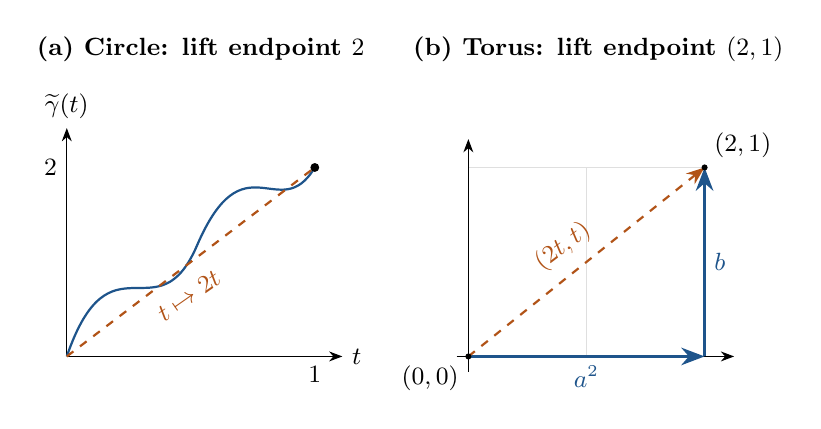
\begin{tikzpicture}[font=\small,>=Stealth]
\node[font=\small\bfseries] at (1.7,3.9) {(a) Circle: lift endpoint $2$};
\draw[->] (0,0) -- (3.5,0) node[right] {$t$};
\draw[->] (0,0) -- (0,2.9) node[above] {$\widetilde\gamma(t)$};
\draw[pathblue,thick] (0,0) .. controls (0.55,1.6) and (1.15,0.25) .. (1.65,1.4)
 .. controls (2.25,2.8) and (2.7,1.65) .. (3.15,2.4);
\draw[pathorange,thick,dashed] (0,0) -- (3.15,2.4);
\fill (3.15,2.4) circle (1.6pt);
\node[left] at (0,2.4) {$2$};
\node[below] at (3.15,0) {$1$};
\node[pathorange,rotate=35] at (1.55,0.77) {$t\mapsto 2t$};
\node[font=\small\bfseries] at (6.75,3.9) {(b) Torus: lift endpoint $(2,1)$};
\begin{scope}[xshift=5.1cm,x=1.5cm,y=2.4cm]
\draw[step=1,gray!25,very thin] (0,0) grid (2,1);
\draw[->] (-0.1,0) -- (2.25,0);
\draw[->] (0,-0.08) -- (0,1.15);
\draw[pathblue,very thick,->] (0,0) -- (2,0);
\draw[pathblue,very thick,->] (2,0) -- (2,1);
\draw[pathorange,thick,dashed,->] (0,0) -- (2,1);
\fill (0,0) circle(1.1pt) node[below left] {$(0,0)$};
\fill (2,1) circle(1.1pt) node[above right] {$(2,1)$};
\node[pathblue,below] at (1,0) {$a^2$};
\node[pathblue,right] at (2,0.5) {$b$};
\node[pathorange,rotate=37] at (0.8,0.58) {$(2t,t)$};
\end{scope}
\end{tikzpicture}
\caption{Winding separates normal forms because lifts remember endpoints.
Left: a lift beginning at $0$ and ending at $2$ is straightened to $2t$.
Right: the sequential word $a^2;b$ and the simultaneous loop have lifts
with common endpoints $(0,0)$ and $(2,1)$; straight-line interpolation in
$\mathbb R^2$ gives a homotopy after projection to the torus.
Both plots are drawn in the covering spaces $\mathbb R$ and $\mathbb R^2$.}
\label{fig:winding}
\end{figure}


\section{What the Lean developments check}
\label{sec:formalization}

\paragraph{Realization model boundary.}
The manuscript's trace carrier in Section~\ref{main-sec:traces} uses flat signed
words with equal-duration slots. The earlier Lean modules use parenthesized
traces and recursively apply Mathlib's half-and-half
\LeanName{Path.trans}. Their observable code retains the exact parametrized
realization. Adding the flattened signed word to that code does not remove
the binary timing coordinate. Consequently, the existing Lean topology
theorems concern the binary model. They must not be read as certificates of
the equal-slot observable topology without a separate comparison theorem.
Endpoint-fixed homotopy of the two realizations is sufficient for semantic
soundness, but does not establish such a topological comparison.
The binary development and its verified results are retained. A separate
implementation now defines \LeanName{GeometricTrace.flatRealize} on the same
endpoint-indexed tree carrier. Each positive factor in a concatenation
receives time proportional to its primitive length; zero-length factors are
omitted. The theorem \LeanName{flatRealize_slot} proves, including slot
boundaries and reversal, that letter $i$ occupies exactly
$[i/n,(i+1)/n]$. The theorem \LeanName{flatRealize_eq_of_flatWord} proves
equality of parametrized realizations for trees with the same signed word.
Thus parentheses are invisible to this realization. The theorem
\LeanName{flatRealize_homotopic_binary} supplies the endpoint-fixed homotopy
bridge; it does not compare the two observable quotient topologies.

\LeanName{EqualSlotTopology} defines separate fixed-endpoint and global
observation topologies using this exact flat realization, without retaining
a binary realization coordinate. The coherent carrier can be reused:
\LeanName{coherent_iff} proves that coherence with the binary and flat paths
are equivalent propositions, and \LeanName{scoped_sound} transfers rewrite
soundness. The literal-word bridge now closes the two additional obligations.
\LeanName{LiteralWord.Word.normalization} reconstructs each tree from its
composable signed word using only units, associativity, and reversal laws.
An independently generated word relation uses adjacent-letter cancellation
and the flattened named rules; \LeanName{WordRwEq.ofTrace_iff} proves that it
agrees with tree rewriting. Equality of geometric paths is never introduced
as a rewrite rule.

The literal finite strata have $W_0=X$ and the compatible positive signed
tuples with their product-subspace topologies. Harmless Lean universe lifts
are removed by explicit homeomorphisms. Canonical equal-slot reconstruction
is continuous on every stratum. The coproduct topology is induced by
$(s(p),p)$, where the second coordinate is the complete signed word: the
source retains the basepoint of an empty word. The source coordinate is
redundant on every positive stratum. The theorems
\LeanName{Word.sensitiveTopology_eq_tupleTopology} and
\LeanName{TotalWord.sensitiveTopology_eq_coproductTopology} then identify
the full-word refinements with these genuine literal-word topologies.
Neither result identifies a binary observable topology with a flat one.

\begin{proposition}[binary timing can identify observable codes]
\label{prop:binary-timing-collision}
There is a three-generator based circle presentation with no named rewrite
rules for which the observable quotients of the fixed-base carriers differ:
the binary quotient is not $T_0$, and the equal-slot flat quotient is discrete.
\end{proposition}
\begin{proof}
Let $\alpha(t)=[t]$ in $\Circle$, and let the primitive labels $a,b,c$
realize $\alpha$, $\beta=\alpha\star\alpha$, and
$\chi=\alpha\star\beta$, respectively, with $\star$ denoting ordinary
half-and-half concatenation. The binary traces
$p=(a;b);b$ and $q=c;(a;a)$ both realize $\chi\star\beta$.
They have length three and can choose this same path as coherent
representative, so their binary observable codes agree. Signed occurrence
count of $c$ is invariant under structural scoped rewrites and has values
zero and one on these two traces. Their scoped classes are distinct.
Every open set in the induced raw observable topology contains both chosen
representatives or neither; the same holds for their classes by the
definition of quotient topology. Hence that quotient is not $T_0$.

For the flat construction, the six oriented primitive paths have distinct
winding numbers $1,2,3,-1,-2,-3$. Restriction to each prescribed equal slot
therefore recovers the signed letter. At each fixed length there are finitely
many words, with distinct realizations in the Hausdorff compact-open path
space. This finite image is discrete, so the fiber of each observed word is
open. The discrete length coordinate separates the strata. A scoped-class
preimage is a union of word fibers, even when the coherent path varies;
thus the fixed-base flat quotient is discrete. This last assertion concerns
the quotient of the based carrier, not an unproved subspace comparison with
the global quotient.
\end{proof}

The exact binary collision is implemented in \LeanName{BinaryTimingCollision},
which proves failure of $T_0$ for both the fixed-base trace quotient and the
global binary scoped quotient. Coherent-representative elimination transfers
the fixed-base trace result to the matching coherent quotient. The actual
circle winding computation, flat discreteness, and exclusion of every
binary/flat observable homeomorphism are checked in
\LeanName{FlatObservableDiscreteness.BinaryCircle}.

\begin{proposition}[fixed-endpoint coherent-representative elimination]
\label{prop:coherent-elimination}
For a fixed realization model and endpoints, give traces a topology making
realization continuous and coherent representatives the topology induced by
$(p,\gamma)$. If scoped equivalence depends only on the trace, forgetting
$\gamma$ induces a homeomorphism between the coherent quotient and the
trace-only scoped quotient.
\end{proposition}
\begin{proof}
The projection $r(p,\gamma)=p$ is continuous, and
$s(p)=(p,|p|)$ is a continuous section. Both maps preserve the quotient
relations. We have $r s=\mathrm{id}$, while $s r(p,\gamma)$ is scoped
equivalent to $(p,\gamma)$ because the trace is unchanged. Quotient descent
therefore gives continuous mutually inverse maps. No geometric completeness
hypothesis is needed. Apply the statement separately to each realization
model and each chosen trace topology.
\end{proof}

\LeanName{CoherentRepresentativeElimination} implements this result for
fixed endpoints with the binary observable trace topology and its full-word
refinement. Its general declaration accepts any trace topology for which
the same binary realization is continuous. \LeanName{EqualSlotTopology}
proves the matching result with the equal-slot canonical section, including
the observable trace topology and its full-word refinement. These are
separate fixed-endpoint homeomorphisms. \LeanName{LiteralWord.TotalWord}
extends matching equal-slot elimination and structural reconstruction to
global arrows, and \LeanName{LiteralWord.WordPair} extends them to the quotient
of the actual endpoint-matched representative subspace. Both the observable
and full-word versions are checked; the full-word version is also identified
with the genuine literal-word coproduct. These results do not identify the
ordinary pullback topology, a based subspace inside a global quotient, or a
binary observable topology with a flat one.

\begin{table}[htbp]
\centering\footnotesize
\begin{tabular}{>{\raggedright\arraybackslash}p{0.20\linewidth}
                >{\raggedright\arraybackslash}p{0.27\linewidth}
                >{\raggedright\arraybackslash}p{0.30\linewidth}
                >{\raggedright\arraybackslash}p{0.12\linewidth}}
\toprule
Result & Exact local declaration & Assumptions & Model\\
\midrule
Binary elimination & \LeanName{quotientHomeomorph} &
Fixed endpoints; realization continuous for supplied trace topology;
trace-only scoped relation & Binary\\
Timing collision & \LeanName{realize_eq} &
Any based path; three discrete labels with the stated realizations & Binary\\
Based failure of $T_0$ & \LeanName{fixed_not_t0} &
Same three-label system; no named rewrite rules & Binary\\
Global failure of $T_0$ & \LeanName{not_t0} &
Same three-label system; no named rewrite rules & Binary\\
Exact slot formula & \LeanName{flatRealize_slot} &
Endpoint-indexed trace; index $i<n$ and $t\in I$ & Flat tree\\
Word independence & \LeanName{flatRealize_eq_of_flatWord} &
Fixed endpoints; equal signed words & Flat tree\\
Homotopy bridge & \LeanName{flatRealize_homotopic_binary} &
Any endpoint-indexed trace & Both\\
Flat elimination & \LeanName{quotientHomeomorph} &
Fixed endpoints; flat realization continuous for supplied trace topology & Flat tree\\
Flat discreteness & \LeanName{BinaryCircle.flat_traceQuotient_discrete} &
Circle paths with six distinct oriented realizations; fixed-base carrier & Flat\\
\bottomrule
\end{tabular}
\caption{Model-boundary verification map. The first row is in
\protect\LeanName{CoherentRepresentativeElimination}; the next three are in
\protect\LeanName{BinaryTimingCollision}, all under
\protect\LeanName{ComputationalPaths.Path.GeometricTopology}.
The next three are in \protect\LeanName{GeometricTrace}, and flat elimination
is in \protect\LeanName{EqualSlotTopology}. The flat-discreteness row is in
\protect\LeanName{FlatObservableDiscreteness}. The earlier eight formal rows passed
Lean~4.32.0 kernel checks at source commit
\href{https://github.com/Arthur742Ramos/TopologicalComputationalPaths/tree/404ac0103e48be805f14a0865c128bc2dbfdcac5}
{\texttt{404ac01}}, with Mathlib commit \texttt{81a5d257}; only
\protect\LeanName{propext}, \protect\LeanName{Classical.choice}, and
\protect\LeanName{Quot.sound} occur in their axiom closures.
Flat discreteness and the nonhomeomorphism conclusion are now formalized in
\protect\LeanName{FlatObservableDiscreteness.BinaryCircle}, using winding numbers
of the six actual oriented primitive paths. The earlier manifest
\protect\LeanName{model-boundary-replay.json} at commit \texttt{131e4bf}
selected 19 actual declarations for direct NanoDa replay, accepted in
\href{https://github.com/Arthur742Ramos/TopologicalComputationalPaths/actions/runs/37726628135}
{the exact-head Quality run}. The five earlier Comparator selections
retain their own scopes. Later selections extend this coverage as described
below.}
\label{tab:model-boundary-verification}
\end{table}

The presentation-change milestone adds
\LeanName{ScopedWordInterpretation} and \LeanName{ContinuousWordInterpretation}.
The former checks primitive finite-trace substitutions, named-rule-to-scoped
preservation, primitive roundtrip extension, and the algebraic
\LeanName{quotientEquiv}. The latter checks
\LeanName{WordSubstitution.mapTrace_length},
\LeanName{mapTrace_realize}, and \LeanName{continuous_binary}, and derives
\LeanName{ScopedWordInterpretation.quotientHomeomorph} for supplied trace
topologies and \LeanName{binaryQuotientHomeomorph} under the primitive
conditions of Proposition~\ref{main-prop:word-substitution-criterion}.
\LeanName{RedundantGeneratorObservable.quotientEquiv} checks the conservative
move of Proposition~\ref{main-prop:redundant-generator-observable};
\LeanName{continuous_oldParity}, \LeanName{new_classes_ne},
\LeanName{new_inseparable}, and \LeanName{not_continuous_inverse} check its
topological failure for the fixed-endpoint flat-tree observable quotients.
All these declarations passed the Lean~4.32.0 kernel at source commit
\href{https://github.com/Arthur742Ramos/TopologicalComputationalPaths/tree/d604b75c2f689e57955302475275064167a4116d}
{\texttt{d604b75}}, with the same pinned Mathlib and only the three standard
axioms listed in Table~\ref{tab:model-boundary-verification}.
The expanded direct-replay manifest selects 37 actual declarations;
its hosted acceptance must be checked on the exact published head.
That earlier 37-declaration milestone included no general variable-length
flat invariance, global presentation equivalence, or final-pair transport.
The current milestone adds those results under the primitive-word continuity
hypotheses of Theorem~\ref{main-thm:flat-word-invariance}.


The literal-word milestone adds the checked results in
Table~\ref{tab:literal-word-verification}. All use Lean~4.32.0 with
Mathlib~\texttt{81a5d257}; their axiom closures contain only
\LeanName{propext}, \LeanName{Classical.choice}, and \LeanName{Quot.sound}.
The source snapshot is
\href{https://github.com/Arthur742Ramos/TopologicalComputationalPaths/tree/0346c8e8d87cfca2e41314ed7efa5fe67316acd9}
{\texttt{0346c8e}}. The direct replay manifest selects the
actual declarations; exact-head hosted acceptance is recorded with the
published artifact, separately from local kernel checking.

\begingroup\footnotesize
\setlength{\tabcolsep}{3pt}
\begin{longtable}{>{\raggedright\arraybackslash}p{0.17\linewidth}
                  >{\raggedright\arraybackslash}p{0.37\linewidth}
                  >{\raggedright\arraybackslash}p{0.28\linewidth}
                  >{\raggedright\arraybackslash}p{0.11\linewidth}}
\caption{Literal-word verification map. Names are in
\protect\LeanName{ComputationalPaths.Path.GeometricTopology.LiteralWord}.
Every row has source commit \texttt{0346c8e}.}
\label{tab:literal-word-verification}\\
\toprule Result & Exact declaration & Assumptions & Model\\
\midrule
\endfirsthead
\toprule Result & Exact declaration & Assumptions & Model\\
\midrule
\endhead
Structural normalization & \LeanName{Word.normalization} &
Any continuous scoped presentation; no named rule used & Both\\
Same-word rewriting & \LeanName{Word.scopedEq_of_flatWord} &
Parallel trees with equal signed words & Both\\
Independent relation & \LeanName{WordRwEq.ofTrace_iff} &
Adjacent-letter cancellation and flattened named rules & Literal/\newline tree\\
Stratum execution & \LeanName{Strata.continuous_flatRealize_family} &
Continuous primitive realization; genuinely composable tuples & Flat\\
Initial coproduct code & \LeanName{Strata.totalWordTopology_eq_induced_code} &
Empty basepoint retained; compatible finite tuple strata & Flat\\
Variable-length family & \LeanName{Strata.continuous_flatRealize_of_flatWord} &
Continuous endpoints and full signed word; typed compatibility & Flat\\
Fixed tuple comparison & \LeanName{WordRwEq.tupleQuotientHomeomorph} &
Matching full-word topology and scoped relation & Flat\\
Global comparison & \LeanName{TotalWord.coproductQuotientHomeomorph} &
Matching equal-slot coherent carrier and literal coproduct & Flat\\
Final-pair comparison & \LeanName{WordPair.coproductQuotientHomeomorph} &
Quotient of actual composable representative subspace & Flat\\
Discrete full-word quotient & \LeanName{discrete_traceSensitiveQuotient} &
Fixed endpoints and discrete labels; alphabet need not be finite & Flat\\
\bottomrule
\end{longtable}
\endgroup

\begingroup\footnotesize
\setlength{\tabcolsep}{3pt}
\begin{longtable}{>{\raggedright\arraybackslash}p{0.15\linewidth}
                  >{\raggedright\arraybackslash}p{0.39\linewidth}
                  >{\raggedright\arraybackslash}p{0.29\linewidth}
                  >{\raggedright\arraybackslash}p{0.09\linewidth}}
\caption{Presentation invariance and separation verification map.
Names are under \protect\LeanName{ComputationalPaths.Path.GeometricTopology}.
Every row has source commit \texttt{0346c8e}.}
\label{tab:invariance-separation-verification}\\
\toprule Result & Exact declaration & Assumptions & Model\\
\midrule
\endfirsthead
\toprule Result & Exact declaration & Assumptions & Model\\
\midrule
\endhead
Word substitution & \LeanName{FlatWordSubstitution.continuous_substitution} &
Continuous primitive word codes; arbitrary finite output lengths & Flat\\
Fixed invariance & \LeanName{ScopedWordInterpretation.flatSensitiveQuotientHomeomorph} &
Rule preservation; primitive roundtrip rewrites; continuous word codes & Flat\\
Global invariance & \LeanName{ScopedWordInterpretation.flatSensitiveGlobalHomeomorph} &
Same hypotheses; common ambient space & Flat\\
Final-pair invariance & \LeanName{ScopedWordInterpretation.flatSensitiveFinalPairHomeomorph} &
Same hypotheses; actual matching-endpoint representative subspace & Flat\\
Projection compatibility & \LeanName{ScopedWordInterpretation.finalPairMap_left},
\LeanName{ScopedWordInterpretation.finalPairMap_right} & No ordinary product-quotient hypothesis & Flat\\
Abbreviation invariance & \LeanName{RedundantGeneratorObservable.flatSensitiveGlobalHomeomorph},
\LeanName{RedundantGeneratorObservable.flatSensitiveFinalPairHomeomorph} & Discrete old and new alphabets; the actual defining rule & Flat\\
Timing nonhomeomorphism & \LeanName{FlatObservableDiscreteness.BinaryCircle.binary_flat_not_homeomorphic} &
Actual three-label circle paths; fixed endpoints; no named rules & Both\\
Complete presentation & \LeanName{CompleteDiscreteSeparation.complete} &
All continuous paths as discrete labels; homotopy named rules & Both\\
Ordinary quotient recovery & \LeanName{CompleteDiscreteSeparation.observableHomeomorph} &
Any based topological space; compact-open path topology & Flat\\
Complete separation & \LeanName{CompleteDiscreteSeparation.not_homeomorphic} &
Ordinary based quotient explicitly assumed nondiscrete & Flat\\
\bottomrule
\end{longtable}
\endgroup

The current direct-replay manifest selects 178 actual declarations (127 theorems
and 51 definitions), extending the 141-declaration represented-rose selection. Its
source and dependency closure are audited against the manifest before NanoDa
replay. Only \LeanName{propext}, \LeanName{Classical.choice}, and
\LeanName{Quot.sound} are permitted. The exact published-head Quality run
checks these declarations separately from the five retained Comparator
selections. The rose development adds an actual geometric carrier and a
checked Cayley-edge covering to the reduced-word calculation. It proves
completeness between represented traces, geometric noncommutation, and
discreteness of the two fixed-endpoint flat computational quotients.
The all-loop extension constructs an actual continuous contraction of that
covering realization, derives simple connectivity, and classifies arbitrary
continuous rose loops by reduced words. Its multiplication convention and
realization comparison are explicit in Table~\ref{tab:rose-all-loop-verification}.

\begingroup
\footnotesize
\setlength{\tabcolsep}{3pt}
\begin{longtable}{>{\raggedright\arraybackslash}p{0.16\linewidth}
                 >{\raggedright\arraybackslash}p{0.32\linewidth}
                 >{\raggedright\arraybackslash}p{0.29\linewidth}
                 >{\raggedright\arraybackslash}p{0.15\linewidth}}
\caption{Geometric rose verification map. Every name has prefix
\protect\LeanName{ComputationalPaths.Path.GeometricTopology}.
The source snapshot is
\href{https://github.com/Arthur742Ramos/TopologicalComputationalPaths/tree/dbfe65efd2deec99cf42df2999f6a20d63c63c23}
{\texttt{dbfe65e}}, with Lean~4.32.0 and Mathlib \texttt{81a5d257}.
The listed results use only the three permitted standard axioms.}
\label{tab:rose-verification}\\
\toprule Result & Exact declaration & Assumptions & Model\\
\midrule
\endfirsthead
\toprule Result & Exact declaration & Assumptions & Model\\
\midrule
\endhead
Actual rose & \LeanName{GeometricRose.axesHomeomorph} &
Two additive circles, exactly their zero points glued & Geometric\\
Reduced normal form & \LeanName{RoseReducedWords.normalization},
\LeanName{RoseReducedWords.scoped_iff_encode_eq} &
Any two based primitive loops; no named rewrites & Scoped algebra\\
Geometric covering & \LeanName{CayleyRoseCovering.covering} &
Actual interval-glued free-group edges; proved quotient and orbit fibers & Geometric\\
Computed endpoint & \LeanName{RoseLiftedWords.liftPath_trace_one} &
Actual rose primitives and covering; identity starting vertex & Binary path\\
Trace completeness & \LeanName{RoseLiftedWords.trace_complete},
\LeanName{RoseLiftedWords.flat_trace_complete} &
Based finite traces; actual endpoint-fixed homotopy & Binary and flat\\
Order separation & \LeanName{RoseLiftedWords.ab_not_homotopic_ba} &
Actual once-around primitive loops & Geometric\\
Signed observation & \LeanName{RoseBasedTopology.signedPrimitive_injective} &
The four actual oriented paths; winding pairs through retractions & Parametrized\\
Based quotients & \LeanName{RoseBasedTopology.flatObservableHomeomorph},
\LeanName{RoseBasedTopology.flatSensitiveHomeomorph} &
Fixed endpoints; respective proved discrete quotient topologies & Flat\\
Tree prefix step & \LeanName{CayleyReducedPrefix.outward_word_cases} &
Actual reduced free-group words; no geometric assumptions & Algebraic\\
\bottomrule
\end{longtable}
\endgroup

Two Lean developments accompany the paper.  The parent artifact
(Section~\ref{sec:parent-artifact}) uses Lean 4.24.0 and Mathlib 4.24.0 and covers the constructions
listed in Table~\ref{tab:declarations}.  A smaller extraction, built with
Lean~4.32.0, contains one bundled statement registered in Palomar
(Section~\ref{sec:palomar}).  The statements and proofs in this paper can be read without
either implementation, and in both cases the checks cover the named
declarations and nothing else.

\begingroup
\footnotesize
\setlength{\tabcolsep}{3pt}
\begin{longtable}{@{}p{.20\textwidth}p{.33\textwidth}p{.24\textwidth}p{.16\textwidth}@{}}
\caption{All-loop rose verification map. Names have prefix
\protect\LeanName{ComputationalPaths.Path.GeometricTopology}.
The source snapshot is
\href{https://github.com/Arthur742Ramos/TopologicalComputationalPaths/tree/3fd21d0ab730b80efc26002084b52bd430a919d4}{\texttt{3fd21d0}}; Lean~4.32.0,
Mathlib \texttt{81a5d257}; only the three permitted standard axioms.}
\label{tab:rose-all-loop-verification}\\
\toprule Result & Exact declaration & Assumptions & Model\\
\midrule
\endfirsthead
\toprule Result & Exact declaration & Assumptions & Model\\
\midrule
\endhead
Exact edge timing & \LeanName{CayleyFlatWalk.walkPath_prefix},
\LeanName{CayleyFlatWalk.outward_last_edge},
\LeanName{CayleyFlatWalk.inward_last_edge} & Actual signed geometric edges;
reduced-word prefix proved & Flat\\
Joint contraction & \LeanName{CayleyContraction.continuous_contract},
\LeanName{CayleyContraction.homotopy} & Actual closed-edge quotient;
local compactness of the compact Hausdorff interval & Geometric tree\\
Simple connectivity & \LeanName{CayleyContraction.contractible},
\LeanName{CayleyContraction.simplyConnected} & Constructed homotopy;
no simple-connectivity input & Geometric tree\\
Full fundamental group & \LeanName{RoseFundamentalGroup.fundamentalGroupEquiv},
\LeanName{RoseFundamentalGroup.freeGroupEquiv} & Concrete covering;
proved simple connectivity & Opposite $F_2$, then inversion\\
Every continuous loop & \LeanName{RoseFundamentalGroup.loop_homotopic_flat_decode},
\LeanName{RoseFundamentalGroup.loopWord_eq_iff_homotopic} & Any actual based
continuous loop & Flat; endpoint-fixed homotopy\\
Realization comparison & \LeanName{RoseFundamentalGroup.traceQuotientEquiv_flat_mk},
\LeanName{RoseFundamentalGroup.traceQuotientEquiv_mul} & Structural scoped rules;
explicit opposite multiplication & Flat; algebraic quotient\\
\bottomrule
\end{longtable}
\endgroup

\subsection{The parent artifact}
\label{sec:parent-artifact}

\paragraph{Traces, soundness, and quotient operations.}
The implementation represents traces by the parenthesized inductive type
\LeanName{GeometricTrace}, where Section~\ref{main-sec:traces} uses flat signed words.  The
declarations \LeanName{WeightedSlotReparam},
\LeanName{balancedSlotReparam}, and
\LeanName{weightedConcatenationInvariant} relate the parametrizations up to
endpoint-fixed homotopy, including the null-homotopy assumptions needed when
a factor has zero weight. They do not identify observable topologies.
The scoped-rewrite modules check soundness and the quotient operations.  The
comparison with Mathlib's fundamental groupoid identifies the represented
homotopy classes, checks preservation of identities, inverses, and
composition, and proves that the induced map on final composable-pair domains
is continuous.

\paragraph{Representative topologies.}
The module \LeanName{TraceSensitiveTopologicalCompPath} flattens internal
traces to signed words while retaining binary realization in its observable
coordinate. It checks continuity of that binary realization, of the map to
observable coordinates, and of the identity, reversal, and binary composition
operations. The earlier quotient modules still use the
observable topology by default.

The module \LeanName{TraceSensitiveSeparation} checks the two-label
separation mechanism on a finite code space: the one-letter trace codes
differ, their observable codes agree, and the identity from the discrete
trace topology to the indiscrete observable topology is continuous while its
inverse is not. It also checks that the two circle labels realize the same
nonconstant loop, proves the signed-count invariant for every structural
scoped rewrite, and separates their scoped quotient classes. Their full
observable codes agree. Signed count descends continuously to the
trace-sensitive quotient; the comparison to the observable quotient is
continuous, but its inverse is not. Thus the topological separation in
Example~\ref{main-ex:quotient-topology-separation} is checked in Lean. The module
\LeanName{TraceSensitiveUniversalCollapse} checks the continuous one-letter
section and the homeomorphism between the two universal quotient topologies.
The abstract mechanism of Proposition~\ref{main-prop:complete-trace-separation}
is checked in \LeanName{CompleteDiscreteSeparation}. Its labels are all
continuous interval paths, with a separate discrete label topology, and its
named rules are exactly homotopies of parallel realized traces. The global
geometric-completeness criterion is proved directly. For based loops at a fixed $x$,
\LeanName{observableHomeomorph} identifies the flat observable quotient with
the ordinary quotient fundamental group, while \LeanName{sensitive_discrete}
proves discreteness of the full-word quotient for the possibly infinite
alphabet. With nondiscreteness of the ordinary based quotient as an explicit
hypothesis, \LeanName{not_homeomorphic} excludes every homeomorphism between
the two topologies. Matching coherent-representative versions are checked too.
The harmonic archipelago and Fabel's facts about its based quotient remain
external mathematical inputs; no such facts are introduced as Lean axioms.

\paragraph{Circle and torus examples.}
The module \LeanName{FiniteCircleTorusPresentation} uses one circle generator
and two torus generators.  It checks integer and integer-pair codes for
traces, completion certificates, and soundness of the torus commuting square.
The modules \LeanName{BasedScopedTraceGroup},
\LeanName{FiniteCircleScopedCompleteness}, and
\LeanName{FiniteTorusScopedCompleteness} prove normalization for the exact
finite presentations. The circle proof uses only the structural groupoid
laws; the torus proof adds its single named commuting square. Both prove
based geometric completeness, instantiate the trace-topology comparison,
and identify the based scoped quotients with discrete $\mathbb Z$ and
$\mathbb Z^2$, respectively. Composing with the geometric winding
homeomorphisms gives explicit homeomorphisms from the scoped based quotients
to the ordinary circle and torus loop quotients.
The separate torus development in
\LeanName{ComputationalPaths/Path/Topology/TopologicalTorusScoped.lean}
includes the comparison between simultaneous and sequential loop
representatives.

\paragraph{Hawaiian-earring transfer.}
The dedicated module checks that an externally supplied failure of the
product-quotient property yields failure of ordinary-pair compatibility, and
it transfers discontinuity of multiplication along the comparison
homeomorphism.  Fabel's results enter as assumptions; the Lean development
does not reprove them.

\paragraph{Build and archive.}
The root import file is \LeanName{ComputationalPaths.lean}, and
Table~\ref{tab:declarations} in Appendix~\ref{app:declarations} lists the
principal declarations.  The core artifact, version
\texttt{0.6.1+lean-only-v3}, is archived on Zenodo under the version DOI
\href{https://doi.org/10.5281/zenodo.21938980}
{\nolinkurl{doi:10.5281/zenodo.21938980}}; its concept DOI is
\href{https://doi.org/10.5281/zenodo.21817207}
{\nolinkurl{doi:10.5281/zenodo.21817207}} \cite{RamosEtAl2026TopologyArtifact}.
The source, including the finite-generator module, the torus
simultaneous/sequential bridge, and the trace-sensitive topology module, is
also in the
\href{https://github.com/Arthur742Ramos/ComputationalPathsLean}{GitHub repository}.
Build the project with \texttt{lake build}; the artifact README lists commands
for building individual modules separately.

The checked modules contain no unfinished proofs and no custom axiom
declarations.  Declaration-level axiom inspection reports only Lean's standard
logical and quotient principles: propositional extensionality, classical
choice, and quotient soundness.  The development complements earlier work on
computational paths and the Lean theorem prover
\cite{deMoura2021,RamosEtAl2025LeanPreprint,RamosEtAl2025OmegaPreprint}.

\subsection{The registered result}
\label{sec:palomar}
The extraction
\href{https://github.com/Arthur742Ramos/TopologicalComputationalPaths}
{\emph{TopologicalComputationalPaths}} has a registered Palomar result,
\href{https://palomar-registry.org/entry?id=PALOMAR-2026-08-29-000005&version=1}
{\texttt{PALOMAR-2026-08-29-000005}}, version~1,
published on 29~August~2026 \cite{PalomarScoped2026}.
It selects the single bundled declaration
\LeanName{TopologicalComputationalPaths.main_result} at the immutable commit
\[
 \texttt{8254c40d0de03ff469c7c9c05087b8bc154e9a87},
\]
built with Lean~4.32.0 and its checked-in dependency manifest.  The selected
statement is an \LeanName{OrdinaryTopologyComparisonCertificate}, and
Table~\ref{tab:palomar-scope} summarizes what it covers.

The certificate has three parts.  The first gives the continuous bijection
between final and ordinary pair spaces, the equivalent criteria for their
topologies to agree, the compact-Hausdorff and discrete sufficient
conditions, the consequence for ordinary composition, and the obstruction
obtained from discontinuity.  (The discrete field assumes that both
$G_{\mathcal P}$ and its final domain are discrete; by
Corollary~\ref{main-cor:discrete} the first assumption implies the second.)  The
second part classifies based-loop homotopy classes of the circle and torus by
integers and integer pairs.  It checks the invariant, the standard
representatives, the identity value, additivity under concatenation, and that
the classification maps are mutually inverse.  The homeomorphism statements
of Theorems~\ref{thm:circle-winding} and~\ref{thm:torus-winding} are not part
of it.  The third part transfers the Hawaiian-earring obstruction under the
hypotheses described below.

\begin{table}[htbp]
\centering\small
\begin{tabular}{>{\raggedright\arraybackslash}p{0.27\linewidth}
                >{\raggedright\arraybackslash}p{0.65\linewidth}}
\toprule
Part of the paper & Scope of the registered certificate\\
\midrule
Final/ordinary comparison &
Canonical continuous bijection; exact quotient/homeomorphism/topology
criteria; sufficient conditions and ordinary-composition consequence.\\
Circle and torus &
Additive classifications of the actual loop quotients, with explicit
standard representatives and inverse laws.\\
Hawaiian earring &
Concrete observable based fiber and quotient comparison; obstruction
transfer conditional on \LeanName{FabelHawaiianEarringFacts}.\\
Broader exposition &
Not certified by this selection: the trace-sensitive refinement, the
minimal finite-generator rewrite algorithms, the homeomorphism statements
for the circle and torus, the explanatory homotopies and figures, and the
manuscript as a whole.\\
\bottomrule
\end{tabular}
\caption{What the Palomar registration covers.  Supporting code and
mathematical exposition are listed apart from the selected conclusions.}
\label{tab:palomar-scope}
\end{table}

The Hawaiian-earring field needs a caveat.  In the registered statement, the
topology \LeanName{hawaiianObservableOpenFiberTopology} is induced by the
geometric projection alone, and its one-letter section identifies its
quotient with the standard loop quotient.  This topology was defined for the
registered based-fiber result; identifying it with the topologies of
Section~\ref{main-sec:traces} would need a proof.  The field \LeanName{hawaiian_based_fiber}
assumes \LeanName{FabelHawaiianEarringFacts}, so the failure of the
product-quotient property and the discontinuity of multiplication are
hypotheses there, and the extraction does not reprove them.  In the
mathematical account, Proposition~\ref{main-prop:hawaiian-earring} takes them
from Fabel's published result \cite{Fabel11}.

The current working source after that immutable version equips the Hawaiian
observable based carrier with the topology induced by its full observable
code.  The revised one-letter section and geometric projection are
continuous, and the based quotient remains homeomorphic to the usual loop
quotient.  It also weakens the discrete sufficient condition in the selected
certificate to discreteness of the arrow space alone, and checks continuity
of both projections from the final composable domain.  The present Lean
source also checks the general open-arrow criterion and
Proposition~\ref{main-prop:universal-path-projection}: the path-class projection
is quotient, and its openness implies ordinary multiplication for the
universal presentation. A direct Lean proof now supplies openness under
the hypotheses of Theorem~\ref{main-thm:universal-open-groupoid}. The theorem
itself remains credited to Holkar, Hossain, and Kulkarni.

On fixed endpoint quotients, Lean now identifies the universal based fiber
with the ordinary based-loop quotient.  It proves discreteness, a quotient
pair map, and continuous ordinary multiplication under the semilocal
hypothesis. It also identifies based paths with the endpoint-defined
subspace of the compact-open path space and checks that an open global
projection restricts to an open quotient onto the based-arrow subspace.
For locally path-connected, semilocally simply connected spaces, the checked
open-map theorem removes the remaining hypothesis from that comparison.
The resulting global based-arrow subspace is homeomorphic to the ordinary
based-loop quotient and is discrete.
The module \LeanName{UniversalTotallyDisconnected} proves the unconditional
case of Corollary~\ref{main-cor:totally-disconnected-universal}. Its projection is
a homeomorphism, and ordinary composition is continuous.
\LeanName{EndpointVaryingLadder} establishes the local ladder step: every
path has a compact-open neighborhood whose members differ by short endpoint
connectors. \LeanName{EndpointAbsorption} first gives the center path positive
constant tails. It then inserts connectors confined to suitable endpoint
neighborhoods and proves, by an explicit reparametrization, that the new
path has the required concatenation homotopy class. The module
\LeanName{UniversalSemilocallySimplyConnected} uses both lemmas to show that
the saturation of any compact-open set is open. It also records ordinary
pair compatibility, continuous composition, and the global based-fiber
homeomorphism as consequences.
The integer-indexed scoped circle presentation has a checked normal form;
its fixed endpoint quotient is homeomorphic to $\mathbb Z$, and a continuous
winding-based trace choice identifies its trace-sensitive and observable
quotient topologies.  This integer-indexed certificate is distinct from the
finite-generator circle presentation in Section~\ref{main-sec:circle-torus}.
The current source also checks the general trace-section criterion, the
universal trace collapse, a finite separation model, and the realized
fundamental-groupoid arrow comparison.  For products it defines the
horizontal and vertical continuous step system, checks geometric soundness
of primitive interchange, and proves sorting and based trace completeness
for the presentation in Theorem~\ref{thm:product-completeness}. The module
\LeanName{ProductPrimitiveInterchange} derives the whole-trace rule from
primitive rectangles, shows that the two presentations induce the same
scoped rewrite relation, and transfers based completeness to the smaller
presentation.
For the finite-generator circle and torus, it checks the continuous
winding-based choices of signed traces and proves the required based
completeness for their exact scoped rules. The resulting based quotient
homeomorphisms and trace-topology comparisons are unconditional. A comparison
with the subspace fibers of their global arrow quotients is also checked:
translation of a variable-basepoint loop to zero gives a continuous winding
map on each global scoped quotient, and finite based completeness makes its
restriction to the actual based-arrow subspace injective. The resulting
subspaces are homeomorphic to $\mathbb Z$ and $\mathbb Z^2$, respectively,
and thus to the ordinary geometric loop quotients.
The Lean source for these working results is available at
\href{https://github.com/Arthur742Ramos/TopologicalComputationalPaths/tree/09b20abe0a4f69b361846c2466bff8528044fa93}
{\LeanName{TopologicalComputationalPaths} commit \texttt{09b20abe0a4f69b361846c2466bff8528044fa93}}.
With the repository's Lean~4.32.0 toolchain and checked-in Mathlib manifest,
\texttt{lake build} checks the development and all configured targets.  The
manuscript source, bibliography, and figures are in
\LeanName{paper/topological} and \LeanName{paper/refs.bib}; the manuscript is
not itself a theorem selected by Comparator.
None of these working-source additions has been registered as a new Palomar
version. The internal \LeanName{comparator-roadmap.json} bundle selects a
24-field certificate containing the checked semilocal and totally disconnected
universal cases, product results, finite global fibers, and trace-topology
comparisons. Its Challenge imports the
substantive development, and its Solution assembles the proved declarations.
Comparator, NanoDa, and Lean's kernel replayed this bundle in CI. Palomar's
current Challenge provenance rule excludes local imports, so the bundle is
not a candidate for registration. A separate Mathlib-only Challenge in
\LeanName{comparator-registry-roadmap.json} selects the open-arrow
ordinary-pair quotient, continuity transfer for multiplication, and the
ordinary geometric circle and torus loop-quotient homeomorphisms. These four
statements have not undergone Palomar's mechanical preflight or external
review. The finite scoped global-fiber results remain outside that selection.

To reproduce the registered version~1 result, check out its pinned commit and run
\texttt{lake build}.  The selection file \LeanName{comparator.json} pairs
\LeanName{Challenge.lean} with \LeanName{Solution.lean}.  The theorem
placeholder in \LeanName{Challenge.lean} states what is checked against the
proof in \LeanName{Solution.lean}, so it does not count as an unfinished
proof.  Later follow-up and preimage-solver development is outside this
registered snapshot.  Registration gives a versioned verification record for
the selected formal statement and nothing more.  It does not cover the prose
or the illustrations, and it implies neither journal acceptance nor an
endorsement of novelty.
\FloatBarrier

\section{Declaration index for the parent artifact}\label{app:declarations}
This index records the representative declarations discussed in Section~\ref{sec:parent-artifact}.
It describes the parent Lean artifact, not the independently registered
Palomar selection of Section~\ref{sec:palomar}.  Fully qualified names are retained for
source lookup.
\begingroup
\small
\renewcommand{\arraystretch}{1.0}
\begin{longtable}{>{\raggedright\arraybackslash}p{0.23\linewidth}>{\raggedright\arraybackslash}p{0.69\linewidth}}
\caption{Representative declarations in the parent artifact, not the Palomar selection.}\label{tab:declarations}\\
\toprule
Mathematical layer & Representative checked declarations\\
\midrule
\endfirsthead
\multicolumn{2}{l}{\small\itshape Table \thetable\ continued}\\
\toprule
Mathematical layer & Representative checked declarations\\
\midrule
\endhead
\bottomrule
\endfoot
Scoped syntax and soundness &
\LeanName{ScopedGeometricRewritePresentation},
\LeanName{ScopedRwEq}, \LeanName{ScopedRwEq.sound}\\
Weighted realization &
\LeanName{WeightedSlotReparam}, \LeanName{balancedSlotReparam},
\LeanName{weightedConcatenationInvariant}\\
Trace-sensitive topology &
\LeanName{TraceSensitiveTopologicalCompPath.lean},
\LeanName{continuous_fullTraceRealization},
\LeanName{continuous_traceSensitive_to_observable},
\LeanName{traceSensitiveTopologyCertificate},
\LeanName{TraceSensitiveQuotient.continuous_quotientComparison},
\LeanName{TraceSensitiveQuotient.quotientComparisonHomeomorph_of_realization_section}\\
Finite topology separation &
\LeanName{TraceSensitiveSeparation.oneLetter_e_ne_f},
\LeanName{TraceSensitiveSeparation.observableCode_e_eq_f},
\LeanName{TraceSensitiveSeparation.not_continuous_observable_to_trace},
\LeanName{TraceSensitiveSeparation.certificate}\\
Quotient groupoid and topology &
\LeanName{ScopedComposableClass},
\LeanName{scopedCompositionOnStrong},
\LeanName{scopedFinalTopologicalGroupoidCertificate}\\
Ordinary/final comparison &
\LeanName{scopedProductCompatibility_iff_four_way},
\LeanName{scopedProductCompatibility_of_compact_final_t2}\\
Comparison and normal forms &
\LeanName{ComparisonFunctorCertificate},
\LeanName{comparisonHomeomorph_of_complete},
\LeanName{ScopedGeometricNormalFormCertificate}\\
Universal and obstruction cases &
\LeanName{universalHomeomorph},
\LeanName{ScopedGeometricRewrite.universalTraceSensitiveHomeomorph},
\LeanName{QuotientObstructionTransfer},
\LeanName{MultiplicationComparison}\\
Finite-generator presentation data &
\LeanName{FiniteCircleTorusPresentation.circleFinitePresentation},
\LeanName{FiniteCircleTorusPresentation.circleCompletionEquivInt},
\LeanName{FiniteCircleTorusPresentation.torusFinitePresentation},
\LeanName{FiniteCircleTorusPresentation.torusCompletionEquivIntProd},
\LeanName{FiniteCircleTorusPresentation.torusFiniteCommutingSquare}\\
Completed circle and topological torus &
\LeanName{circleBasedNormalFormCertificate},
\LeanName{TopologicalTorus.standardLoop_homotopic_sequentialLoop},
\LeanName{TopologicalTorus.equivIntProd},
\LeanName{TopologicalTorus.certificate}\\
\end{longtable}
\endgroup

\bibliographystyle{amsplain}
\begingroup\small\bibliography{../refs}\endgroup
\end{document}
